\documentclass{beamer}

\usepackage{amssymb,amsmath}
\usepackage{relsize}
\usepackage{hyperref}
\usepackage{minted}
\usepackage{color}

\title{Herbie}
\subtitle{or: what to do if you can't stop worrying and hate floating point}
\author{Sharif~Olorin \url{<sio@tesser.org>}}
\institute{Ambiata}

\newcommand\Bibfont{\fontsize{6pt}{7.2}\selectfont}

\begin{document}

\frame{\titlepage}

\begin{frame}[fragile]

\frametitle{Arithmetic quiz}

\begin{minted}[mathescape]{haskell}
sum :: [Double] -> Double
\end{minted}

\end{frame}

\begin{frame}[fragile]

\frametitle{Arithmetic quiz}

\begin{minted}[mathescape]{haskell}
sum :: [Double] -> Double
sum = foldl (+) 0.0
\end{minted}

\end{frame}

\begin{frame}[fragile]

\frametitle{Arithmetic quiz}

\begin{minted}[mathescape]{haskell}
sum :: [Double] -> Double
sum = foldl (+) 0.0 . sort
\end{minted}

\end{frame}

\begin{frame}[fragile]


\frametitle{Arithmetic quiz}


\begin{minted}[mathescape]{haskell}
sum :: [Double] -> Double
sum [] = 0.0
sum xs =
  uncurry go $ bisect xs
  where
    go [y] [] = y
    go [] [z] = z
    go [y] [z] = y + z
    go ys zs =
      let (y1s, y2s) = bisect ys
          (z1s, z2s) = bisect zs in
      (go y1s y2s) + (go z1s z2s)

    bisect ws =
      let len = length ws `div` 2 in
      (take len ws, drop len ws)
\end{minted}

\end{frame}

\begin{frame}[fragile]

\frametitle{Arithmetic quiz}

\begin{minted}[mathescape]{haskell}
sum :: [Double] -> Double
sum = fst . foldl add (0.0, 0.0)
  where
    add (acc, err) x =
      let
        -- Correct for the error from the last iteration.
        y = x - err
        acc' = acc + y
        -- Algebraically, err' should be zero.
        err' = (acc' - acc) - y
      in (acc', err')
\end{minted}

\end{frame}

\begin{frame}[fragile]
\frametitle{A cautionary tale}

\begin{minted}[mathescape]{haskell}
stddev :: Double -> Double
stddev variance = sqrt $ abs variance
\end{minted}

\end{frame}

\begin{frame}[fragile]
\frametitle{A cautionary tale}

\begin{minted}[mathescape]{haskell}
stddev :: Double -> Double
stddev variance = sqrt $ abs variance
\end{minted}

\[\sigma_{1:n}^2 = \frac{1}{n} \sum\limits_{i=1}^n (x_i - \mu_{1:n})^2\]

\end{frame}

\begin{frame}[fragile]

\frametitle{Refresher on IEEE 754}
  
\[F = \{s \times b^e | s, e \in \mathbb{Z}; b \in \mathbb{N} \}\]

\begin{itemize}
\item In general, arithmetic operations are commutative but not associative.
\item Common causes of error are subtracting very similar values and
  adding very different values.
\item Multiplication, squaring et cetera can compound existing error.
\item Rounding contributes at most 0.5 ULPs (units in the last place)
  of error per operation.
\end{itemize}

\end{frame}

\begin{frame}[fragile]

\frametitle{Refresher on IEEE 754}

\[ n \cdot \frac{1}{n} = 1 \]

\begin{minted}[mathescape,frame=lines,escapeinside=||]{haskell}
  |$\lambda$| let n = 10
  |$\lambda$| sum . replicate n $ 1 / n
  0.9999999999999999
\end{minted}

\[ x + y - x = y \]

\begin{minted}[mathescape,frame=lines,escapeinside=||]{haskell}
  |$\lambda$| let x = 10**(-10)
  |$\lambda$| let y = 10**20
  |$\lambda$| printf "%f, %f\n" y z
  0.0000000001, 100000000000000000000.0
  |$\lambda$| printf "%f\n" $ y + x - y
  0.0
\end{minted}

\end{frame}  

\begin{frame}

\frametitle{What is error?}

\[\epsilon(x, y) = \log_2 | { z \in FP | min(x, y) \leq z \leq max(x,y) } |\]

\begin{itemize}
  \item Error in ULPs: number of floating-point values between the
    exact result and the approximate result\cite{schkufza2014}.
  \item Consistent representation of error independent of magnitude.
  \item The binary log approximates ``number of incorrect bits''.
\end{itemize}
\end{frame}

\begin{frame}
  \frametitle{Herbie}
  \begin{itemize}
  \item Provides automated synthesis of more accurate versions of
    floating-point computations\cite{panchekha2015}.
  \item Written by Pavel Panchekha et. al. at the University of Washington.
  \item Around 10KLOC of Racket.
  \item Intended for scientists, statisticians, people who don't
    necessarily have a background in numerical analysis.
  \end{itemize}
\end{frame}

\begin{frame}
  \frametitle{Herbie}
  \begin{figure}
    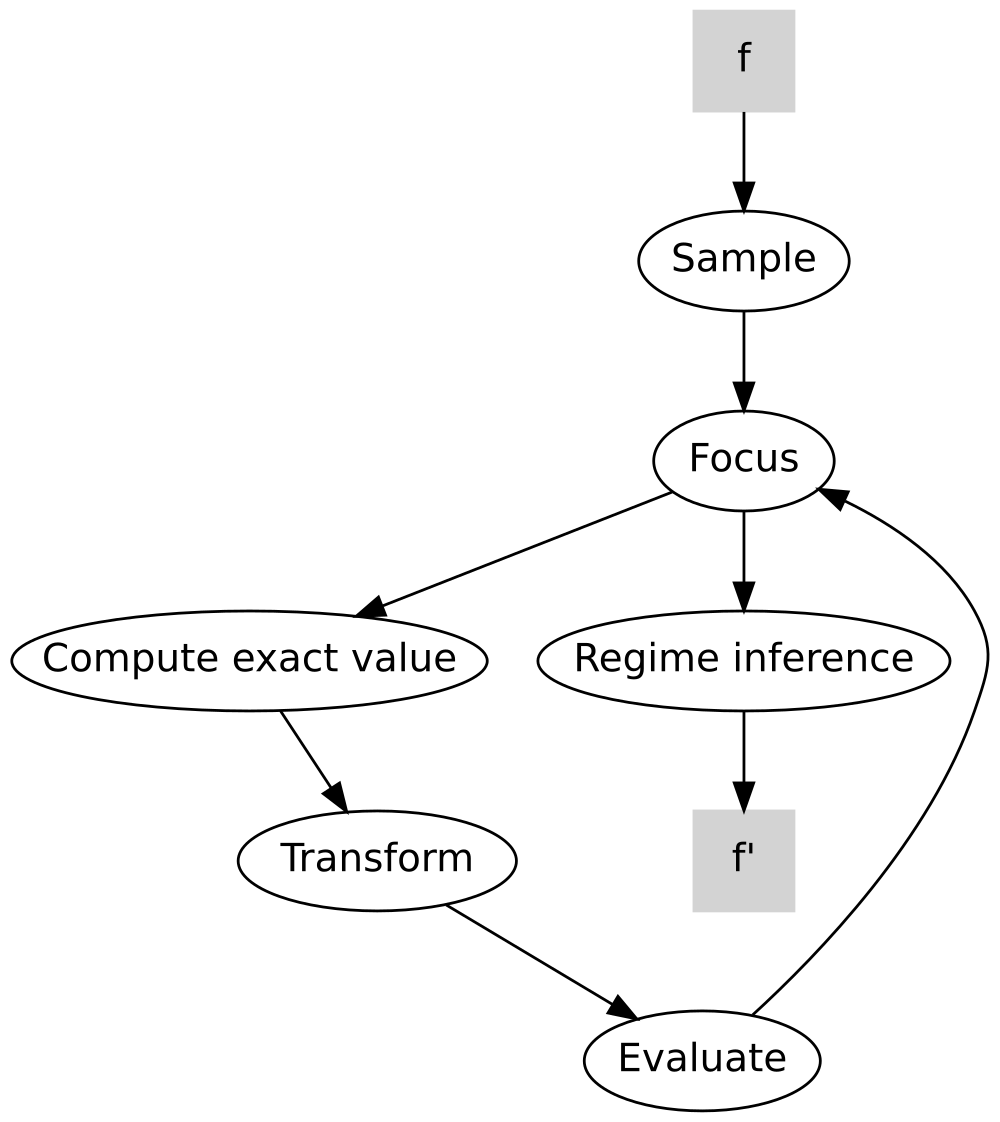
\includegraphics[scale=0.55]{img/loop.png}
  \end{figure}
\end{frame}

\begin{frame}
  \frametitle{Sample}
  \begin{itemize}
    \item Sample inputs are drawn uniformly from the computation's
      domain.
    \item Herbie defaults to 256 samples per iteration.
    \item More samples leads to greater probability of identifying
      regions of the domain with differing error behaviour.
  \end{itemize}
\end{frame}

\begin{frame}
  \frametitle{Error and input domain}

  \begin{figure}
    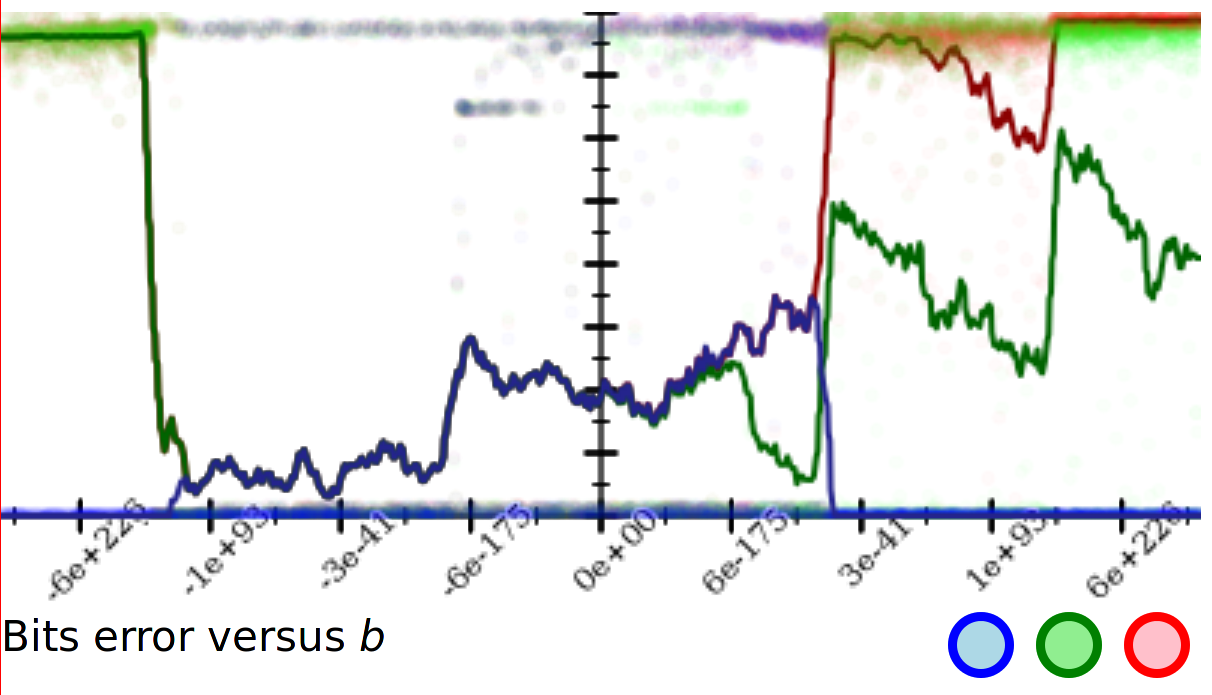
\includegraphics[scale=0.2]{img/quadratic-b}
    \caption{Herbie's error estimates for the quadratic formula \( \frac{-b + \sqrt{b^2 - 4ac}}{2a} \)}
  \end{figure}
\end{frame}

\begin{frame}
  \frametitle{Focus}

  \[ \frac{-b + \sqrt{\color{blue} b^2 \color
      {red} - \color{blue} 4ac}\color{black}}{2a} \]

  \begin{itemize}
  \item For each operator \( \star \), evaluate operands \( a \) and
    \( b \) in exact arithmetic for all of the sampled inputs.
  \item Evaluate \( a \star b \) in both exact arithmetic and
    floating-point arithmetic.
  \item Focus search on operators which contribute the most error.
  \end{itemize}


\end{frame}

\begin{frame}
  \frametitle{``Exact'' results}

  Even with arbitrary precision, how do you know how many bits are
  ``enough''? Herbie guesses:

  \begin{itemize}
    \item Compute the result with \(n\) bits of precision over your
      entire sample.
    \item Do it again with \(2n\) bits.
    \item If the most significant 64 bits of the results match, this
      is your exact answer; otherwise continue.
  \end{itemize}
\end{frame}

\begin{frame}
  \frametitle{Transform}
  \begin{itemize}
  \item Hill-climbing greedy search of a database of rewrite rules.
    \begin{itemize}
    \item \(x^2 - y^2 \leadsto (x - y)(x + y)\)
    \end{itemize}
  \item Transformations are either mathematical identities or
    near-identities - sometimes using an approximation can result in a
    numerical result closer to the true value.
  \item Followed by a series-expansion pass.
    \begin{itemize}
      \item \(e^x - 1 \leadsto x + \frac{1}{2}x^2 + \frac{1}{6}x^3\) for \(x \approx 0\)
    \end{itemize}
  \item Simplification phase to cancel like terms, et cetera -
    pattern-match expressions which can be reduced.
    \begin{itemize}
      \item \(\frac{y}{e^{x - x}} \leadsto y\)
    \end{itemize}
  \end{itemize}
\end{frame}

\begin{frame}
  \frametitle{Regime inference}
  \begin{itemize}
  \item Many computations have error characteristics which vary based
    on the magnitude of the input within the domain (``regime'').
  \item This necessitates the selection of different implementations
    at runtime based on the value of the inputs, as no single formula
    will be accurate in all cases.
  \item Herbie localises regime boundaries using the segmented least
    squares dynamic programming algorithm\cite{kleinberg2006}.
  \item To avoid overfitting, a penalty is added when evaluating each
    segmentation - one bit of error per branch.
  \end{itemize}
\end{frame}

\begin{frame}[fragile]
  \frametitle{A simple example}
  \[\sqrt{x} - \sqrt{x - 1}\]

  \begin{minted}[mathescape,frame=lines]{racket}
  (herbie-test (x)
    "Subtracting square roots"
    (- (sqrt x)
       (sqrt (- x 1))))
  \end{minted}
\end{frame}

\begin{frame}
  \frametitle{A simple example}
  \begin{figure}
    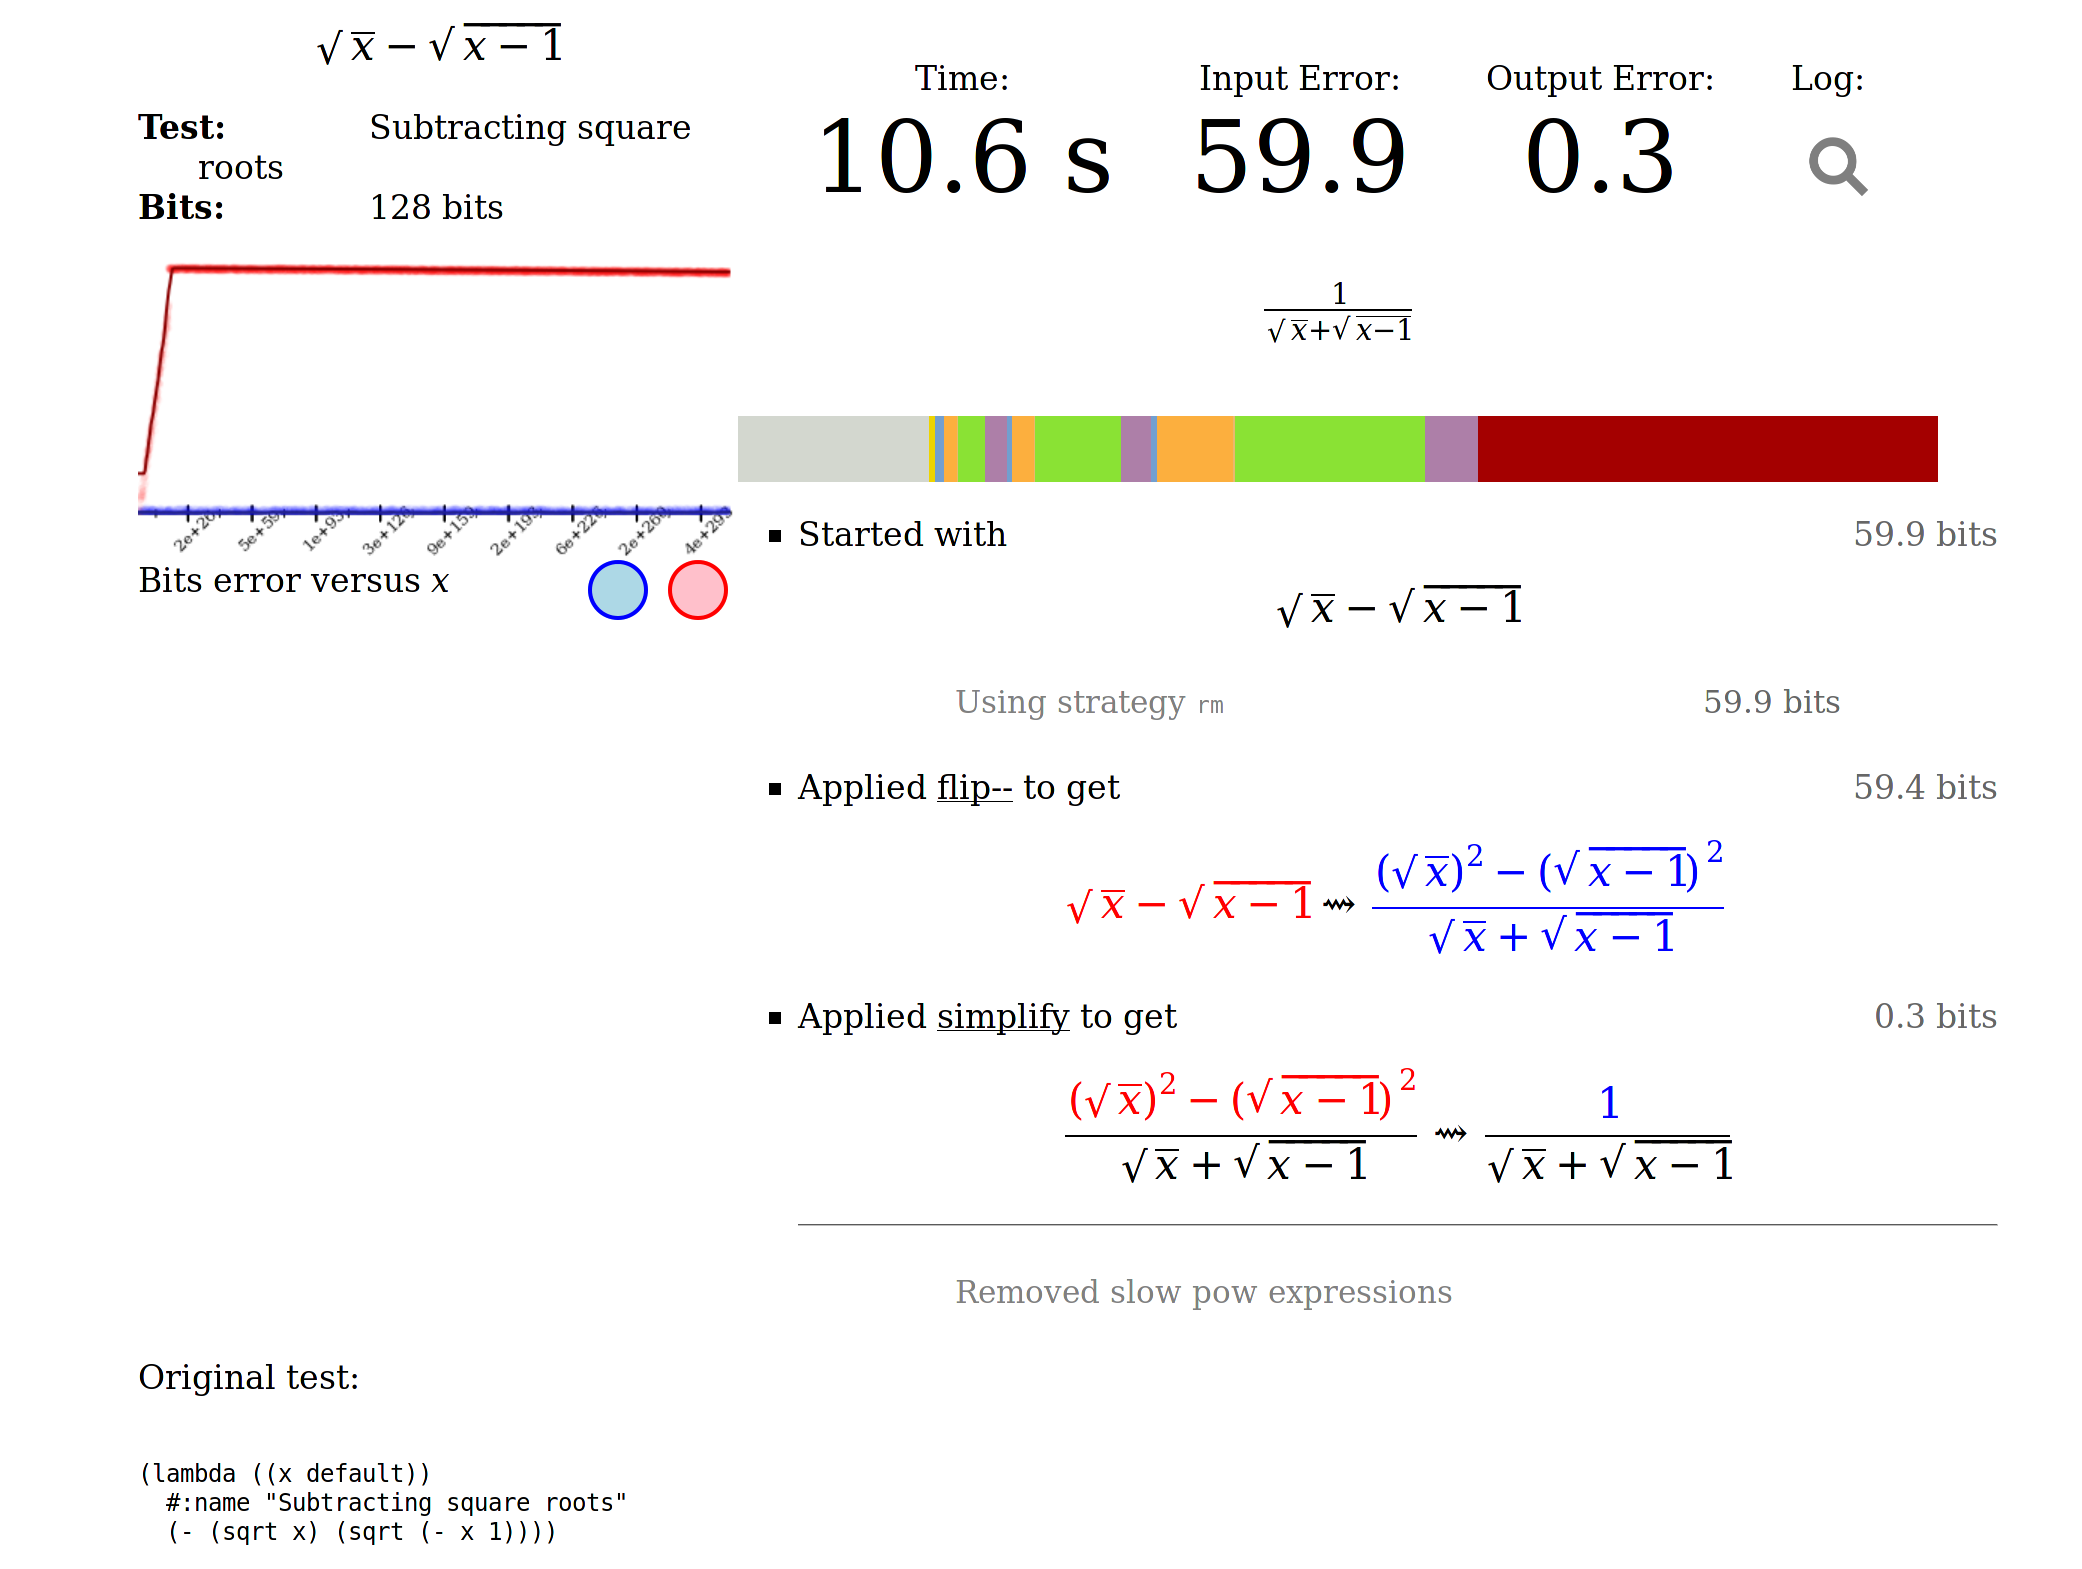
\includegraphics[scale=0.12]{img/simple-example}
    \caption{Herbie report for difference of square roots.}
  \end{figure}
\end{frame}

\begin{frame}
  \frametitle{Combining variance of subsamples}
  \[\sigma_{1:n+m}^2 = \frac{m(\sigma_{1:m}^2 + \mu_{1:m}^2) + n(\sigma_{m+1:n}^2 + \mu_{m+1:n}^2)}{m + n} - \mu_{1:n+m}^2\]
  \begin{itemize}
  \item \(\sigma_{a:b}^2\) is the variance of the subsample from
    values \(a\) to \(b\).
  \item \(\mu_{a:b}^2\) is the mean of the subsample from values \(a\)
    to \(b\).
  \end{itemize}
\end{frame}

\begin{frame}[fragile]
  \frametitle{Combining variance of subsamples}

  \begin{minted}[mathescape,frame=lines]{racket}
(herbie-test (mu
              mu1
              [var1 (uniform 0 100000000)]
              [n (< 0 int)]
              mu2
              [var2 (uniform 0 100000000)]
              [m (< 0 int)])
    "Combine variance of subsamples"
    (- (/ (+ (* n (+ var1 (sqr mu1)))
             (* m (+ var2 (sqr mu2))))
          (+ n m))
       (sqr mu)))
  \end{minted}
\end{frame}

\begin{frame}
  \frametitle{Combining variance of subsamples}
  \begin{figure}
    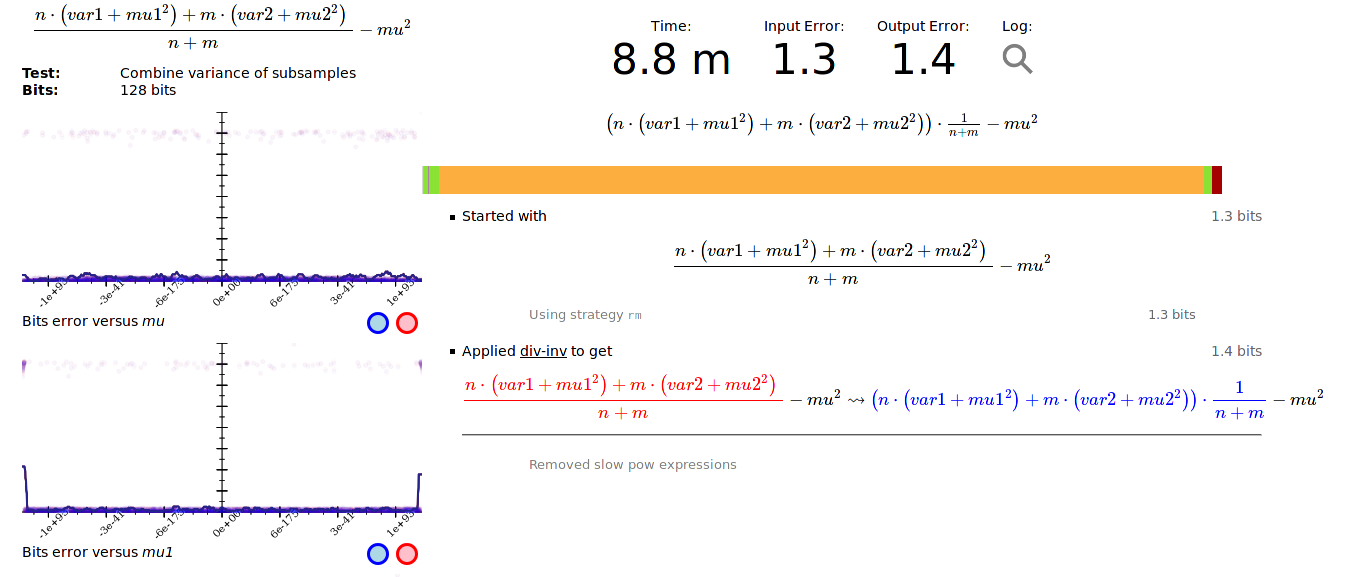
\includegraphics[scale=0.24]{img/subsamples}
    \caption{Herbie report for combining subsample variance.}
  \end{figure}
\end{frame}


\begin{frame}
  \frametitle{Miscellanea}
  \begin{itemize}
  \item Herbie: \url{https://github.com/uwplse/herbie}
  \item GHC plugin: \url{https://github.com/mikeizbicki/HerbiePlugin}
  \item Rust plugin: \url{https://github.com/mcarton/rust-herbie-lint}
  \item Valgrind plugin: \url{https://github.com/uwplse/herbgrind}
  \item These slides: \url{https://tesser.org/doc/slides/2016-05-25-fp-syd-herbie.pdf}
  \end{itemize}
\end{frame}


\begin{frame}
\frametitle{Bibliography}

\Bibfont

\bibliographystyle{plain}
\bibliography{slides.bib}
\end{frame}

\end{document}
